%\documentclass[11pt]{scrartcl}
\documentclass[11pt]{scrreprt}

\usepackage[T1]{fontenc}
\usepackage[utf8]{inputenc}
% \usepackage[ngerman]{babel}

\usepackage{graphicx}
\graphicspath{ {../resources/imgs/} }

%\usepackage[backend=biber, style=ieee]{biblatex}
\usepackage[backend=bibtex, style=authoryear-comp]{biblatex}
%\newcommand{\citep}{\parencite}  % adds \citep alias for citing with parenthesis
\let\citef\cite  % makes \citef an alias for \cite
\let\cite\parencite  % makes \cite an alias for \parencite
\addbibresource{../resources/MA.bib}

\KOMAoptions{parskip=half}

\usepackage[margin=3cm]{geometry} % Adjust margins

\usepackage{soul}
\usepackage{todonotes}
\usepackage{amsmath}
\usepackage{hyperref}
\usepackage{cleveref}
\usepackage{caption}
\usepackage{subcaption}
\usepackage{booktabs}
\usepackage{rotating}
\usepackage{pdfpages}
\usepackage{csquotes}
\usepackage{algorithm}
\usepackage{algpseudocode}

\usepackage{array}  % needed for '\newcolumntype' command
\newcolumntype{L}[1]{>{\raggedright\arraybackslash}p{#1}}  % define "L" column type


\usepackage{newfloat}
\DeclareFloatingEnvironment[
  listname = {List of Patterns} ,
  name = Pattern,
  placement = h,
  within = none
]{pattern}

\usepackage{newfloat}
\DeclareFloatingEnvironment[
  listname = {List of Hyperedges} ,
  name = Hyperedge,
  placement = h,
  within = none
]{hedge}

\Crefname{pattern}{Pattern}{Patterns}
\crefname{pattern}{pattern}{patterns}
\Crefname{hedge}{Hyperedge}{Hyperedges}
\crefname{hedge}{hyperedge}{hyperedges}


\usepackage{lipsum}  % produces dummy text


\begin{document}


% ========== Title page

\titlehead
{
\begin{tabular}{ll}
\begin{minipage}{0.5\textwidth}
	\textbf{Technische Universität Berlin} \\
	Fakultät IV: Elektrotechnik und Informatik \\
	Institut für Telekommunikationssysteme \\
	Fachgebiet Verteilte offene Systeme	
\end{minipage}
&
\begin{minipage}{0.5\textwidth}
	\raggedleft
	
\includegraphics[width=0.3\textwidth]{logos/tub_logo_bw.jpg}			
\end{minipage}

\end{tabular}
}

\subject{Masters Thesis in Computer Science}
\title{Extending Semantic Hypergraphs by Neural Embedding-based Semantic Similarity for Pattern Matching}
\author{Max Reinhard \\ \small Matrikelnummer: 359417}

\date{\today}
\publishers{Supervised by Prof. Dr. Manfred Hauswirth \\
	Additional guidance by Prof. Dr. Camille Roth\thanks{Centre Marc Bloch (An-Institut der Humboldt-Universität zu Berlin)} \\ 
	and Dipl.-Math. Thilo Ernst\thanks{Fraunhofer-Institut für offene Kommunikationssysteme}}
	
\maketitle

% ========== Abstract
\begin{abstract}
\textbf{Abstract}
\lipsum[1-2]
\end{abstract}

% ========== TOC
\tableofcontents
\newpage

% ========== Body
% ==============================

% ========== 
\chapter{Introduction}
\begin{itemize}
	\item Context: The big problem
	\item Problem statement: The small problem
	\item Methodology / Strategy
	\item Structure
\end{itemize}

\textbf{Notes:}
\begin{itemize}
	\item Huge amounts of text, which can provide insight about stuff
	\item Automatic tools can provide assistance for humans to process all the text
	\item This generally means filtering the original text corpus or otherwise reducing amount of information the information that has to be processed by humans
	\item Filtering introduces a bias
	\item Especially for scientific purposes it is relevant to mitigate bias or at least understand what bias has been introduced (to make it transparent)
	\item Semantic Hypergraphs can be a valuable tool for that because...
\end{itemize}


Human life in times of widespread use of the internet and smartphones is most certainly more than ever interspersed with text-based communication...


A Semantic Hypergraphd \cite{menezes_semantic_2021} is a form of representation for Natural Language (NL) and therefore knowledge. \textit{NL} sentences can be modelled as a recursive hypergraph which can be represented in a formal language. The framework allows to specify semantic patterns in this formal language which can be matched against an existing \textit{SH}.

The aim of the SH framework is to provide a \textit{open} and \textit{adaptive} framework to analyse text corpora, especially in the domain of computational social science (CSS) \cite{lazer2009computational}. The framework is \textit{open} in the sense that it's representation formalism is inspectable and intelligible by humans and that the pattern matching follows explicit rules. The framework is adaptive in the sense that the parsing is based on adaptive subsystems (ML-based) and therefore allows for an error-tolerant parsing from \textit{NL} to \textit{SH} in regards to grammatical and syntactical correctness (???).




% ========== 
\chapter{Fundamentals and Related Work}
\section{Semantic Hypergraph}

\subsection{Structure}

synonymes: SH, hypergraph, graph.

Edge

Edge Content

Root edge / Sequencen (i use the term "sequence root edge")

\subsection{Syntax / Pattern Matching}

wildcard operator

Variables

Square bracket notation --> word lists

functional patterns -> lemma

> operator for innermost atom


---

Differences between the formal notation and the notation sued in the implementation
(or should this be contained in the implementation chapter?)





\section{Semantic Similarity}

\subsection{Different Similarity Measures}

\subsubsection{String Similarity}
Lievenstein distance, etc..

\subsubsection{Lexical Similarity}
tf-idf, etc.?

\subsection{Types of Semantic Similarity}

\subsubsection{Lexical Databases}
WordNet and alike (not the scope of this work)


\section{Embedding-based Similarity}

\subsection{Embedding Types}

\subsubsection{Fixed Word Embeddings}

\subsubsection{Contextual Ebeddings}

%\subsubsection{Sentence embeddings}

\subsection{Distance Measures}

Mean reference vector vs. pairwise distance

% ========== 
\chapter{Problem Statement}
\label{cha:problem-statement}
CSS researches may typically be interested in retrieving statements of specific kind from a text corpus, such as expressions of sentiment of an actor towards some entity or expressions of conflicts between different actors. One approach for performing the retrieval would be to use a system which allows to specify some form of pattern which abstractly represents the statements they are trying to capture. This requires the definition of some form of formal pattern language\footnote{The \textit{Google Search} query language can be seen as a simple example of such a pattern language, albeit with a different use case focus: \url{https://support.google.com/websearch/answer/2466433?hl=en}} and possibly the prior transformation of the text corpus into some form of structured format to match against. Another approach is to use a system, which accepts example statements concretely representing the statements that are desired to be retrieved. Those systems may require a large number of positive and negative examples to be able to perform the retrieval. The two types of retrieval systems described here are in tendency situated in the realms of symbolic IR/IE and probabilistic ML/DL respectively.

The SH framework is more situated in the former symbolic realm. In SH text is represented in the form of \textit{hyperedges} (in the following also referred to as \textit{edges} only). These edges are either atomic or they consist of edges themselves, which essentially accounts for the recursive character of the SH. Each edge has a specific \textit{type} from a set of eight different types of which the most trivial two types are probably \textit{concept} (\textsf{C}) and \textit{predicate} (\textsf{P}). 

Users of the SH framework (e.g. CSS researchers) can define patterns in the SH formalism to match against a text corpus (e.g. a collection of news articles) that has previously been parsed as an SH. These patterns may among other things specify the structure of the edges that should match it as well as their type (and the types of possible sub-edges). Additionally the actual words that should match need to be specified i.e. the content to match against, if the structure of an edge matches the pattern. 
There are additional operators in the pattern language such as the wildcard operator \textsf{*}, which can be used e.g. to match every atomic edge edge of a specific type and therefore discard content.

To better illustrate the problem \cref{hed:ann-likes-bananas} and \cref{hed:ann-likes-apples} demonstrate how NL sentences are parsed to SH based on this simplified introduction the the SH representation.

\begin{hedge}
  \normalfont\sffamily
  \centering
  ( likes/P ann/C apples/C ) 
  \caption{SH representation for the sentence "Ann likes apples"}
  \label{hed:ann-likes-apples}
\end{hedge}

\begin{hedge}
  \normalfont\sffamily
  \centering
  ( likes/P ann/C bananas/C ) 
  \caption{SH representation for the sentence "Ann likes bananas"}
  \label{hed:ann-likes-bananas}
\end{hedge}

\cref{hed:ann-likes-apples} and \cref{hed:ann-likes-bananas} both follow the same structure, but differ in the content of the last sub-edge. Both edges are hence matched by \cref{pat:ann-likes-something}, which does not specify content for this sub-edge.
The SH pattern language also allows to define a pattern that matches both \cref{hed:ann-likes-apples} and \cref{hed:ann-likes-bananas} via a list of words as in \cref{pat:ann-likes-apples-and-bananas}. However is not possible define a pattern that matches based on some form of \textit{Semantic Relatedness} (SR) or \textit{Semantic Similarity} (SS) \cite{harispeSemanticSimilarityNatural2015} regarding content.
Referring to the example above this means using the SH framework it is not directly possible to to retrieve every sentences that declares that "Ann likes \textit{some kind of fruit}" or that "Ann likes \textit{fruits similar to apples}". This former would require to provide a comprehensive list of every fruit while the latter would require the user to specify all fruits he deems similar to apples.

\begin{pattern}[h!]
  \normalfont\sffamily
  \centering
  ( likes/P Ann/C */C )
  \caption{"Ann-likes-something" pattern}
  \label{pat:ann-likes-something}
\end{pattern}

\begin{pattern}[h!]
  \normalfont\sffamily
  \centering
  ( likes/P ann/C [apples, bananas]/C )
  \caption{"Ann likes apples or bananas" pattern}
  \label{pat:ann-likes-apples-and-bananas}
\end{pattern}

Utilizing some form of SR/SS regarding to edge content for the matching step would allow users to define more generalising patterns. There exists a great variety of approaches for determining the SR/SS of text, which can generally be divided into \textit{Corpus-based Measures} and \textit{Knowledge-based measures} \cite[Section~1.3.2]{harispeSemanticSimilarityNatural2015}. The latter approaches may generally provide the explicitness in the measurement determination that is desired by CSS researchers. However among the former recent ML-based and especially DL-based approaches have been outperforming most other approaches \cite{chandrasekaranEvolutionSemanticSimilarity2021}. They generally rely on computing a vector space representation (or embedding) of texts which can then be used to calculate their similarity and will therefore be referred to as \textit{Neural Embedding-based Semantic Similarity} (NESS) measures in the following. 

Word semantics generally depend on textual context and hence does the SS between words \cite[Section~2.2.3]{harispeSemanticSimilarityNatural2015}. Incorporating contextuality when extending the SH pattern matching process by SS therefore poses a central challenge. Context-dependent SS would allow to specify matching edge content beyond isolated word semantics, although this may not always be desirable or necessary as in the example above. 

As illustrated earlier, NESS measures principally do not provide the explicitness that is inherent to the pattern matching process of the SH framework. In the sense of the adaptive-open classification described above an integration of NESS would mean a shift from openness to adaptivity in this regard. While the SH framework generally can be situated in the realm of symbolic approaches, this integration would build a bridge between it and the realm of probabilistic approaches.

% ========== 
\section{Research Questions}
\label{sec:research-questions}
Based on the problem statement outlined above, we pose the following research questions:

\subsection{Primary Question}
\textbf{R} Can neural embedding-based semantic similarity regarding edge content be be integrated into the pattern matching of the Semantic Hypergraph framework to allow for more generalising patterns while providing control over the adaptiveness and therefore loss of explicitness in the matching process?

\subsection{Secondary Questions}
\textbf{R.1} What neural embeddings model would be the most suitable for accurately assessing semantic similarity within the Semantic Hypergraph pattern matching process while effectively addressing the challenges posed by contextuality?

\textbf{R.2} To what extent does incorporating neural embedding-based semantic similarity improve the generalization performance (recall) and how does it impact precision when matching a pattern against a set of known desired matching results?

\textbf{R.3} How can adaptiveness and explicitness of the matching process be effectively and transparently balanced and controlled?


% ========== 
\chapter{Solution Approach}
\label{cha:solution-approach}
In this chapter we present the approach that was developed to answer the research questions (see \cref{sec:research-questions}). Therefore trying to provide a solution to the problem of extending the SH framework by Neural Embedding-based Semantic Similarity Matching, which is described in \cref{cha:problem-statement} where the relevancy of this problem for has also been derived.

The system is described here will in the following be referred to as \textit{Neural Embedding-based Semantic Similarity extended Semantic Hypergraph Pattern Matching} or:
\begin{center}
\textit{\textbf{NESS-SHPM}} aka \textit{\textbf{NESSeSHyPaM}}	
\end{center}




\section{Integration into the Pattern Matching Process}
\subsection{\texttt{semsim} Functional Pattern}
pattern works only for atoms

\subsection{Sub-pattern Similarity Thresholds}


\section{Fixed Word Embedding-based Matching}
(FNESS)
 
word2vec via gensim

discussion about using transformer models for single word embeddings?


reference words: single-word and multi-word reference

\label{sec:semsim-multi-word}
Square bracket notation 

\section{Contextual Embedding-based Matching}
\textit{Contextual Neural Embedding-based Semantic Similarity} 
(CNESS)


i generally like your idea of contrasting the discrete and continous space as it allows to point out that there cant be one single point, also for a set of words which represents the meaning, but rather some subspace depending on the specific context
Regarding the point of the semantic entities in continuous space being either word- or phrase based, the important difference is, that in case of semsim with context we do not compare the embedding representation of the phrases themselves. rather the sententences/phrases influence the embedding representations of the word (or maybe phrases)
 I tend to see this a bit like a blurring algo. The meaning of each token starts bleeding into its neighbours.


reference edges

\subsection{Context References}
\subsection{Token Mapping}



\section{Similarity Threshold Control}

\subsection{Breakpoint Discovery}
detect change points in number of matches \\ 
see https://github.com/deepcharles/ruptures

half-max point and quarter/three-quarter points (percentiles, not quantiles)
fit function and search for infliction as well as maximum derivative points,
problematic in cases with less continuous change in number of matches.

how to approach this for practical applications?


% ========== 
\chapter{Implementation}
\label{cha:implementation}

\section{Relevant external Software Libraries used}
Here list libs and models to be referenced later.

Word2Vec
Gensim
SentenceTransformers
Transformers
SpaCy

\section{Modules newly added to the SH Framework}
Semsim instances

reference edge sample modification parameter


\section{Modifications of the SH Pattern Matching}
skip semsim

\section{Modifications to the Hypergraph database}
is this really necessary? tok pos etc, but not actually specific to semsim


%\section{SH Notation}
%Bracket notation for multi-word Semsim


%\section{Similarity Threshold}
%\label{sec:similarity-threshold}


%\section{Tokenization}
%
%\subsection{SpaCy}
%SpaCy linguistic tokenization (https://spacy.io/usage/linguistic-features how-tokenizer-works)
%spacy (without transformers) uses an purely rule based (but language depended) tokenizer as far as I understand: https://spacy.io/usage/linguistic-features how-tokenizer-works (the call it linguistic tokenizer)
%
%side note about using different transformer models than the provided one (because i was always confused about this):
%it it possible to exchange the underlying transformer component for basically every transformer model (as long as it follows the conventions that spacy expects), but you would have to retrain the spacy model to be able to use the task specific heads (like e.g. NER)
%footnote: https://github.com/explosion/spaCy/discussions/10327
%
%an alignment is provided between the transformer-tokenizer and the spacy-tokenizer
%lib: https://github.com/explosion/spacy-alignments
%
%footnote: https://explosion.ai/blog/spacy-transformers
%
%
%\subsection{WordPiece and SentencePiece}
%
%SentencePiece: https://github.com/google/sentencepiece


%\section{Matching candidate edge and reference edge tokens}
%both edges should match the pattern and should act as a valid ref edge for each other
%but it is obvious that the tok_idx_trail that leads to the predicate in the one edge wont lead to the predicate in the other edge
%that was the premise on which i built the matching (and which we discussed i think)
%
%so there are 2 cases:
%[candidate edge is more specific than reference edge] the location trail of the token in the candidate edge is longer than in the reference edge. this case should be trivial. we can just cut off the location trail when we reach an atom in the reference tok_pos.
%[reference edge is more specific than candidate edge] the location trail of the token in the candidate edge does not lead to an atom in the reference edge. in this case there is not enough information to match the tokens. i see two possible solutions:
%use the whole sub-edge to compute the reference embedding (maybe i misunderstood and that was your conception all along)
%try to get the information which token to use in some other way. possibly by matching via the atom types… this should work for cases like predicates but would not work if we are looking for a modifier or something else which can appear multiple times. i have the feeling that this should be recoverable through the graphbrain matching process somehow, i just don’t know how….
%(edited)
%
%for now i have the tendency to implement 2a as it is much easier not sure about the semantic implications though




% ========== 
\chapter{Evaluation}
In this chapter the conceived concept (see \cref{cha:solution-approach}) and specific implementation (see \cref{cha:implementation}) of the NESS-SHPM system is being evaluated to answer the research question(s) posed in \cref{sec:research-questions}. Therefore a a case study is conducted to evaluate the system for a specific use case. In this case study quantitative results as well as qualitative examinations of the behaviour of NESS-SHPM are conducted. The quantitative results reflect the systems performance using metrics which are established for retrieval and classification tasks. The qualitative results exemplary showcase detailed aspects of the systems behaviour in the given use case.
\todo{refer to the RQs more specifically?}

\section{Case Study: Conflicts}
The conflicts case study follows the approach presented in \citef{menezesSemanticHypergraphs2021} where expressions of conflict are extracted from a given SH using a single SH pattern. In their work they build upon the information extracted by the pattern to conduct further analyses, which are not in the scope of this work. Here the evaluation is limited to the task of classifying whether the content of a given edge in the SH is an expression of conflict or not. Or framed differently the task is to to retrieve exactly all those edges whose content is an expression of conflict. The evaluation will compare the retrieval performance of a suitable set of different SH patterns by matching them against a labelled dataset.

\todo[inline]{should I explain why specifically the conflicts and not some other case study (i.e. dataset) --> because there was none... but then I need to show why there was none and what are the criteria for a case study to be suitable to evaluate the system}

\subsection{Expressions of Conflict}
\label{sec:conflict-definition}
An expression of conflict in the context of this case study is defined as a sentence which fulfils the following properties:

\begin{displayquote}
There is a conflict between two explicitly named actors, wherever these actors are mentioned in the sentence; whereby a conflict is defined as antagonizing desired outcomes.
\end{displayquote}

\subsection{Reddit Worldnews Corpus}
The corpus from which those expressions of conflict are retrieved consists of news titles that were shared on the social media platform \textit{Reddit}. Specifically all titles shared between January 1st, 2013 and August 1st, 2017 on \textit{r/worldnews}, which is described as: “A place for major news from around the world, excluding US-internal news.”\footnote{\url{http://reddit.com/r/worldnews}} This corpus contains 479,384 news headers and is in the following referred to as the \textit{Worldnews-Corpus}.

Each of these headers is comprised of a single sentence and is represented as a sequence root edge in the SH constructed from it. In the following this SH is referred to as the \textit{Worldnews-SH}. Parsing errors that may potentially occur during this constructed and can obstruct a correct retrieval of a wrongly parsed edge i.e. wrongly represented sentence. These errors are out of scope of this work. All edges in the Worldnews-SH are assumed to be correctly parsed.

%These are some randomly selected examples from the Worldnews-Corpus:
%\begin{itemize}
%	\item Example
%	\item Example
%	\item Example
%\end{itemize}
%
%\todo{add examples}


\subsection{Semantic Hypergraph Patterns}
\label{sec:sh-patterns}
The SH patterns that are used in this evaluation all have the same general form to isolate the effect of replacing a purely symbolic matching against a specific word or list of words with NESS-SHMP. In this section the general form of these pattern will be described, which entails consequences for the creation of the labelled dataset described in \cref{sec:conflict-dataset}. 

%The retrieval performance of the original purely symbolic pattern defined by \citef{menezesSemanticHypergraphs2021} is compared against the retrieval performance of patterns containing some form of the semsim functional pattern. \todo{remove?}


\subsubsection{Original Conflict Pattern}
\Cref{pat:original-conflict} is originally defined in \citef[p.~22]{menezesSemanticHypergraphs2021} and is therefore referred to as the \textit{original conflict pattern}. It is used to extract conflicts between two parties \textsf{SOURCE} and \textsf{TARGET}, potentially regarding some \textsf{TOPIC}. As mentioned before, the assignment of these variables is irrelevant for this case study.

The original conflict patterns contains two sub-patterns which utilize word lists. These sub-patterns match the trigger sub-edge and predicate sub-edge of a candidate edge respectively and are in following referred to as \textit{trigger sub-pattern} and \textit{predicate sub-pattern}. If not stated otherwise these terms will refer to \cref{pat:original-conflict}. 

\begin{itemize}
	\item \textbf{\textsf{Trigger sub-pattern:}} \textsf{[against,for,of,over]/T}
	\item \textbf{\textsf{Predicate sub-pattern:}}
		\textsf{( PRED/P.{so,x} ) \(\wedge\) \\ ( lemma/J >PRED/P [accuse,arrest,clash,condemn,kill,slam,warn]/P )}
\end{itemize}

In the trigger sub-pattern the content of the candidate trigger sub-edge is directly matched against a list of prepositions, which are in the following referred to as the \textit{conflict prepositions}. In case of the predicate sub-pattern, the word list is matched against the lemma of the innermost atom of the candidate predicate sub-edge, which is always a verb. The list of verbs used here will in the following be referred to as the \textit{conflict verbs}.

\begin{itemize}
	\item \textbf{\textsf{Conflict prepositions:}} against, for, of, over
	\item \textbf{\textsf{Conflict verbs:}} accuse, arrest, clash, condemn, kill, slam, warn
\end{itemize}


\begin{pattern}
  \normalfont\sffamily
  \centering
  ( PRED/P.{so,x} SOURCE/C TARGET/C [against,for,of,over]/T TOPIC/[RS] ) \(\wedge\) \\
  ( lemma/J >PRED/P [accuse,arrest,clash,condemn,kill,slam,warn]/P )
  \caption{Original conflict pattern}
  \label{pat:original-conflict}
\end{pattern}


\subsubsection{Wildcard Conflict Patterns}
\label{sec:wildcard-conflict-patterns}
Replacing either the trigger sub-pattern, the predicate sub-pattern or both of them with a semsim function are the options for utilizing NESS-SHPM in a modified version of \cref{pat:original-conflict} without modifying the general structure of the pattern. To evaluate which of these options are best suited to evaluate the retrieval performance of NESS-SHPM, three \textit{wildcard conflict patterns} are constructed. In these patterns the predicate sub-pattern (\cref{pat:wildcard-pred}) or the trigger sub-pattern (\cref{pat:wildcard-prep}) are replaced by the wildcard operator. 
%or both (\cref{pat:wildcard-pred-prep})

\begin{pattern}
  \normalfont\sffamily
  \centering
  ( PRED/P.{so,x} SOURCE/C TARGET/C [against,for,of,over]/T TOPIC/[RS] ) \(\wedge\) \\ ( PRED/P */P )
  \caption{Predicate wildcard pattern}
  \label{pat:wildcard-pred}
\end{pattern}

\begin{pattern}
  \normalfont\sffamily
  \centering
  ( PRED/P.{so,x} SOURCE/C TARGET/C */T TOPIC/[RS] ) \(\wedge\) \\  ( lemma/J >PRED/P [accuse,arrest,clash,condemn,kill,slam,warn]/P )
  \caption{Trigger wildcard pattern}
  \label{pat:wildcard-prep}
\end{pattern}

%\begin{pattern}
%  \normalfont\sffamily
%  \centering
%  ( */P.{so,x} SOURCE/C TARGET/C */T TOPIC/[RS] )
%  \caption{Predicate and trigger wildcard pattern}
%  \label{pat:wildcard-pred-prep}
%\end{pattern}

\paragraph{Preliminary Evaluation}
The three wildcard conflict patterns are matched against the Worldnews-SH and the number of matches is recorded. Comparing the number of matches of these patterns shows which of the sub-patterns is most influential for the retrieval performance of \cref{pat:original-conflict}. \Cref{tab:wildcard-pattern-evaluation} shows the results of these preliminary evaluations as well as the number of matches that result from matching \cref{pat:original-conflict} against the Worldnes-SH. It can be seen that the choice of conflict verbs is much more influential on the number of matches than the choice of conflict prepositions when compared to the number of matches resulting from the original conflict pattern. While replacing the predicate sub-pattern with a wildcard operator yields an increase with a factor of \(12,45\), replacing the trigger sub-pattern with a wildcard operator only yields and increase with a factor of \(1,07\). 


\begin{table}[h]
\centering
\begin{tabular}{lr}
\toprule
\multicolumn{1}{l}{Pattern name}				& \multicolumn{1}{l}{Number of matches} \\
\midrule
Original conflict pattern					& 5766	\\
Predicate wildcard pattern					& 71804 \\
Trigger wildcard pattern						& 6154	\\
%Predicate and trigger wildcard pattern		& 79431	\\
\bottomrule
\end{tabular}
\caption{Results of matching the wildcard patterns against the Worldnews-SH}
\label{tab:wildcard-pattern-evaluation}
\end{table}



\subsubsection{SemSim Conflict Patterns}
Based on the result of the preliminary evaluation in \cref{sec:wildcard-conflict-patterns}, the predicate sub-pattern of \cref{pat:original-conflict} is replaced by different forms of semsim functional patterns to construct different \textit{semsim conflict patterns}. These patterns are then used to evaluate the effects of utilizing NESS-SHPM. The trigger sub-pattern is not modified to better isolate these effects in comparison to purely symbolic SHPM.

\Cref{pat:semsim-conflict} describes the general form of a semsim conflict pattern. The \texttt{<SEMSIM-FUNCTION>} placeholder is replaced with one of the three implemented semsim functions to construct the \textit{semsim-fix conflict pattern} (\cref{pat:semsim-fix-conflict}), \textit{semsim-fix-lemma conflict pattern} (\cref{pat:semsim-fix-lemma-conflict}) and the \textit{semsim-ctx conflict pattern} (\cref{pat:semsim-ctx-conflict}). As \texttt{<SEMSIM-ARGUMENT>} the conflict verb list is used as similarity reference words in \cref{pat:semsim-fix-conflict} and \cref{pat:semsim-fix-lemma-conflict}, which utilize FNESS. In the semsim-ctx conflict pattern, the wildcard operator is used as \texttt{<SEMSIM-ARGUMENT>} since the necessary reference edges can only be provided via an external parameter and not inside the pattern.


\begin{pattern}[H]
  \normalfont\sffamily
  \centering
  ( PRED/P.{so,x} SOURCE/C TARGET/C [against,for,of,over]/T TOPIC/[RS] ) \(\wedge\)\\ 
  ( \texttt{<SEMSIM-FUNCTION>}/J PRED/P \texttt{<SEMSIM-ARGUMENT>}/P )
  \caption{General SemSim conflict pattern}
  \label{pat:semsim-conflict}
\end{pattern}

\begin{pattern}[H]
  \normalfont\sffamily
  \centering
  ( PRED/P.{so,x} SOURCE/C TARGET/C [against,for,of,over]/T TOPIC/[RS] ) \(\wedge\)\\ 
  ( semsim/J PRED/P [accuse,arrest,clash,condemn,kill,slam,warn]//P )
  \caption{semsim-fix conflict pattern}
  \label{pat:semsim-fix-conflict}
\end{pattern}

\begin{pattern}[H]
  \normalfont\sffamily
  \centering
  ( PRED/P.{so,x} SOURCE/C TARGET/C [against,for,of,over]/T TOPIC/[RS] ) \(\wedge\)\\ 
  ( semsim-fix-lemma/J PRED/P [accuse,arrest,clash,condemn,kill,slam,warn]//P )
  \caption{semsim-fix-lemma conflict pattern}
  \label{pat:semsim-fix-lemma-conflict}
\end{pattern}

\begin{pattern}[H]
  \normalfont\sffamily
  \centering
  ( PRED/P.{so,x} SOURCE/C TARGET/C [against,for,of,over]/T TOPIC/[RS] ) \(\wedge\)\\ 
  ( semsim-ctx/J PRED/P */P )
  \caption{semsim-ctx conflict pattern}
  \label{pat:semsim-ctx-conflict}
\end{pattern}



\subsection{Conflict Dataset}
\label{sec:conflict-dataset}
To conduct an evaluation which assesses the retrieval performance of the NESS-SHPM system it is necessary to have a dataset of edges with labels that state whether an edge is an expression of conflict or not. Since such a dataset does not exists it needs to be constructed. In the following the construction process of this \textit{conflict dataset} (CD), which is used for the evaluation in this case study, and the datasets characteristics are discussed.


\subsubsection{Base Edge Set}
The set of edges that can be retrieved by a conflict pattern, i.e. the original conflict pattern or a semsim conflict pattern is restricted the general form of these patterns. This entails that, given the same SH, every set of matching edges of a pattern of this form will be a subset of the matching edges of the predicate wildcard pattern (\cref{pat:wildcard-pred}). The set of edges resulting form matching this pattern against the Worldnews-SH are therefore used as the \textit{base edge set} (BES) from which the conflict dataset is constructed, instead of the entirety of all the hypergraphs sequence root edges.

Every edge in the BES has a predicate sub-edge that has an innermost atom, which is a verb that has a lemma. In the following this is called the \textit{predicate lemma} of an edge. Each of the edges matching \cref{pat:original-conflict} or a pattern in the form of of \cref{pat:semsim-conflict} therefore corresponds to a predicate lemma.

%Matching \cref{pat:wildcard-pred} against the Worldnews-SH results in \(n_{f} = 69 380\) matching edges. In the following the set of those edges will be referred to as the \textit{full dataset} (FD).\todo{add examples}

\subsubsection{Desired Characteristics}
\label{sec:dataset-characteristics}
To effectively evaluate the effectiveness of the application of NESS by matching a pattern in the form of \cref{pat:semsim-conflict}, the dataset used for this should have the following characteristics:

\begin{itemize}
	\item Contain the largest possible number of unique predicate lemmas
	\item Contain the largest possible number of edges per unique predicate lemma
\end{itemize}

On the one hand it is desired to have as many different unique predicate lemmas as possible in the dataset to be able to evaluate whether NESS can differentiate if a predicate lemma indicates an expression of conflict or not. On the other hand it is desired to have as many different edges per unique lemma as possible in the dataset to be able to evaluate whether CNESS is able to differentiate if edges represent an expression of conflict or not, given that they correspond to the same predicate lemma.

\subsubsection{Construction Process}
To create the labelled CD, the edges of the dataset need to be manually labelled by human annotators, which is labor-intensive. The BSE contains \(n_b=71804\) edges. Due to the time constrains of this work and the limited availability of three annotators, the BSE needs to be subsampled to create the CD. Since the desired characteristics described above relate the the distribution of predicate lemmas, it is relevant to verify that is possible to determine the predicate lemma for all edges in the edge set from which the CD is sampled.

\paragraph{Filtering}
Every edge in the BES theoretically corresponds to a predicate lemma, as stated above. Still it can occur that it is not possible to determine the predicate lemma of a given edge to to implementation issues, which out of scope of this work. In these cases an edge is filtered from the BSE, which results in the \textit{filtered base edge set} (FBES). The FBES contains \(n_{f} = 69 380\) edges. 


\paragraph{Sampling} 
The edges in the full dataset correspond to \(n_{l} = 2195\) unique predicate lemmas. Attaining to the desired dataset characteristics, the number of samples \(n_{s}\) in the subsampled dataset should ideally be a multiple \(m_{l} >= 2\) of \(n_{l}\), so that \(n_{s} = m_{l} \cdot  n_{l}\). This would mean that every predicate lemma contained in the full dataset is statistically represented multiple times in the subsampled dataset.
\todo{add lemma distribution plot}

A dataset size of \(n_{s}=2000\) was chosen, wich means \(m_{l} < 2\) and  \(n_s << n_f\). This entails that a trade-off between the desired dataset characteristics has to be made. To account for this, a sampling method is applied that offers more control over the distribution of predicate lemmas in the subsampled dataset than uniform random sampling does. This sampling method is based on the idea of \textit{Stratified Sampling} \cite{parsonsStratifiedSampling2017} \todo{is this correct?} and is described in detail in \cref{algo:dataset-sampling}. 

The procedure splits the full dataset into multiple bins after the edges are sorted by number of occurrence of their predicate lemma and then uniformly randomly samples from each bin. This method guarantees that predicate lemmas which correspond to a relatively small number of edges in the full dataset will be represented in the subsampled dataset, while still representing the distribution of the full dataset. \todo{do I have to show this in some way? should I then mention it at all?}


\begin{algorithm}
\begin{enumerate}
	\item Create a list of tuples \(t\) of edges and their corresponding predicate lemma: \\ \(L = [(l_k, e_i), ...]\) with \(k \in \{0,...,m\}\) and \(i \in \{0,...,n\}\)
	\item Sort this list by the number of tuples containing a predicate lemma to create the list: \\ \(L_{sort} = [(l_0, e_0), ... (l_m, e_n)]\), so that:
	\begin{itemize}
		\item \(n_k\) is the number of tuples containing a lemma \(l_k\)
		\item \(t_j\) with \(j > i\) is a tuple wich sorted after tuple \(t_i\)
		\item \(n_o >= n_p\) if \(t_i = (l_o, e_i)\) and \(t_j = (l_p, e_j)\)
	\end{itemize}			
	\item Split the list \(L_{sort}\) into \(n_{b}\) bins.
	\item Uniformly sample \(n_{sb}\) tuples from each bin.
	\item Build a set of all edges \(e\) contained in the sampled tuples.
\end{enumerate}
\caption{Dataset sampling algorithm}
\label{algo:dataset-sampling}
\end{algorithm}

The subsampled dataset size resulting from this sampling method is \(n_{s} = n_{b} * n_{sb}\). Given \(n_{s} = 2000\), the values \(n_b = 10\) and \(n_{sb} = 200\) were chosen for sampling the CD.


\paragraph{Labelling}
The labelling task is shared between the three annotators. A given edge will be either labeled as \textit{conflict} or \textit{no conflict} by an annotator following the definition given in \cref{sec:conflict-definition}. Because of the aforementioned time constraints, every edge is only labeled by one annotator. To nonetheless ensure a consistent labelling among all annotators, a set of 50 edge is labelled by all three annotators. Every edge for which a disagreement in labelling occurs between at least two of the annotators, is inspected to reach an agreement on the label. Utilizing this process, the annotators understanding of what constitutes an expression of conflict is refined. Following this preliminary step, the \(n_s\) edges of the dataset are equally distributed among the three annotators and individually labelled by them.

% It was confirmed that the percentage of edges that represent an expression of conflict in relation to all edges in the subset given to an annotator did not vary more than ... among all three annotators.

\subsubsection{Edge Set Comparison}
The CD is the result of the filtering, sampling and labelling described above. The size of the Worldnews-SH, FD and SD are listed in \cref{tab:dataset-descriptions} for comparison, along with the number and percentage of edges which are labelled as an expression of conflict and of those which are not.\todo{add examples}


\begin{table}
\centering
\begin{tabular}{lrrr}
\toprule
\multicolumn{1}{l}{Edge set name}	& \multicolumn{1}{c}{Number of} 		& \multicolumn{1}{c}{Number of} 		& \multicolumn{1}{c}{Number of} \\
\multicolumn{1}{l}{} 				& \multicolumn{1}{c}{all edges} 		& \multicolumn{1}{c}{conflict edges} 	& \multicolumn{1}{c}{no conflict edges} \\
\multicolumn{1}{l}{} 				& \multicolumn{1}{c}{} 				& \multicolumn{1}{c}{(\% of all edges)} & \multicolumn{1}{c}{(\% of all edges)} \\
\midrule
Worldnews-SH						& 479384		& -					& - \\
Base Edge Set (BES)					& 71804		& -					& - \\
Filtered BES (FBES)					& 69380 		& - 					& - \\
Conflict Dataset (CD)				& 2000 		& 599 (29.95 \%) 	& 1401 (70.05 \%) \\
\bottomrule
\end{tabular}
\caption{Number of edges and proportion of labels for the different edge sets}
\label{tab:dataset-descriptions}
\end{table}


\subsection{Evaluation Process}
The evaluation process consists of multiple \textit{evaluation runs}. An evaluation run is described by an \textit{evaluation configuration} consisting of a dataset (which is always the CD in this case study) and an SH pattern which is matched against the dataset. For the semsim conflict patterns the evaluation run is further described by an \textit{NESS configuration}. These configurations specify the properties of the NESS matching. That means the \textit{NESS model} and in the case of CNESS it is also specified which set of reference edges is used and if the \textit{all-tokens} version of the matching is used. \todo{add references to chapter 2}

For each evaluation run the \textit{evaluation metrics} are computed. If the evaluation run corresponds to a semsim conflict pattern, this is done for every similarity threshold \(t_s \in r_t\), where \(r_t\) is the range of similarity thresholds. For all evaluation that are conducted in this case study \( r_t= \{0, 0.01, ...,  0.99, 1\}\) is chosen.

%In the case of the patterns including a form of the semsim functional pattern, the semsim processing is skipped during the actual matching phase and the semsim instances are recorded. This way the semsim matching can be repeated for multiple parameters, i.e. references and similarity thresholds, without the need to repeat the entire matching process. 

\paragraph{Conflict Patterns}
\Cref{sec:sh-patterns} describes the four conflict patterns used in this evaluation in detail and derives why they are chosen. A structured overview of the properties of these patterns can be seen in \cref{tab:evaluation-patterns}.

\paragraph{Reference Edge Sets}
The reference edges are randomly sampled from the set of edges in the CD, which are labelled as "conflict". To account for the effect of different reference edge sets, multiple different samples are drawn. There are five sets of reference edges used in this evaluation, which are listed in the appendix. \todo{create appendix and add reference to it}

\paragraph{Evaluation Configurations}
\Cref{tab:evaluation-run-configs} describes the configurations for all evaluation runs that are conducted in this case study.

\subsubsection{Evaluation Metrics}
Using the information provided by the dataset labels it is determined whether a match is correct or not. If an edge is matches in a given evaluation run and is labeled as "conflict" in the dataset, it is considered a \textit{true positive} (TP). If an edge matches but is labeled "no conflict", it is considered a \textit{false positive} (FP). The \textit{true negatives} (TN) and \textit{false negatives} (FN) are determined analogously  by examining the non-matching edges. Based on the TP, FP, TN and FN the metrics \textit{accuracy}, \textit{precision}, \textit{recall} and \textit{F1 score} are computed.
\todo{leave out accuracy?}

\begin{table}
\centering
\begin{tabular}{lcccc}
\toprule
\multicolumn{1}{l}{Pattern name}		& \multicolumn{1}{c}{Lemma}		& \multicolumn{1}{c}{SemSim}	& \multicolumn{1}{c}{Includes}		& \multicolumn{1}{c}{Requires} \\
\multicolumn{1}{l}{} 				& \multicolumn{1}{c}{based} 		& \multicolumn{1}{c}{type} 		& \multicolumn{1}{c}{ref. words} 	& \multicolumn{1}{c}{ref. edges} \\
\midrule
Original conflict (\cref{pat:original-conflict})					& Yes 		& - 		& -			& - \\
semsim-fix conflict (\cref{pat:semsim-fix-conflict})				& No		& FIXED		& Yes		& No \\
semsim-fix-lemma conflict (\cref{pat:semsim-fix-conflict}) 		& Yes 		& FIXED		& Yes		& No \\
semsim-ctx conflict (\cref{pat:semsim-fix-conflict})				& No		& CONTEXT	& No		& Yes \\
\bottomrule
\end{tabular}
\caption{Properties of the conflict patterns used in the evaluation}
\label{tab:evaluation-patterns}
\end{table}


\begin{table}
\centering
\begin{tabular}{llccc}
\toprule
\multicolumn{1}{l}{Evaluation} & \multicolumn{1}{l}{Conflict} & \multicolumn{3}{c}{NESS Configuration} \\
\cmidrule{3-5}
\multicolumn{1}{l}{Run Name}   & \multicolumn{1}{l}{Pattern}  & \multicolumn{1}{c}{Model}    & \multicolumn{1}{c}{Ref. Edges Sets}	& \multicolumn{1}{c}{Use \textit{all-tokens}} \\
\midrule
original                       	& original                    & -                            & -                                   	& -    \\
semsim-fix w2v                 	& semsim-fix                  & word2vec                     & -                                   	& -    \\
semsim-fix cnb					& semsim-fix                 & cn-nb							& -                                   	& -    \\
semsim-fix-lemma w2v           & semsim-fix-lemma            & word2vec                     & -                                   	& -    \\
semsim-fix-lemma cnb            & semsim-fix-lemma            & cn-nb					& -                                   	& -    \\
semsim-ctx e5                  & semsim-ctx                  & e5                           & -                                   	& No   \\
semsim-ctx gte                 & semsim-ctx                  & gte                          & -                               		& No   \\
semsim-ctx e5 at			& semsim-ctx                  & e5                           & -                                  	& Yes  \\
semsim-ctx gte at			& semsim-ctx                  & gte                          & -                                 	& Yes  \\
\bottomrule
\end{tabular}
\caption{Evaluation Run Configurations}
\label{tab:evaluation-run-configs}
\end{table}


\subsection{Evaluation Results}

\subsubsection{Quantitative Results}
Table XYZ shows results for all evaluation runs. 
best precision, recall and f1 score
for all evaluation runs using NESS, the best score it the score achieved with 







\subsubsection{Qualitative Results}


table with evaluation runs, their 






%To investigate whether it is possible to capture the abstract concept of a country using the multi-word \texttt{semsim} pattern introduced in \ref{sec:semsim-multi-word}, a list of the worlds 20 most populous countries \footnote{Based on \url{https://en.wikipedia.org/wiki/List_of_countries_and_dependencies_by_population}, Accessed on XYZ} is used (listed in descending order by population size):
%
%
%\textit{India, China, USA, Indonesia, Pakistan, Nigeria, Brazil, Bangladesh, Russia, Mexico, Japan, Philippines, Ethiopia, Egypt, Vietnam, Congo, Iran, Turkey, Germany, France}
%
%To avoid the repetition of that list in the following pattern, we introduce a variable:
%
%\begin{pattern}
%  \normalfont\sffamily
%  \centering
%  COUNTRIES = [india,china,usa,indonesia,pakistan,nigeria,brazil,bangladesh,russia,mexico, ajapan,philippines,ethiopia,egypt,vietnam,congo,iran,turkey,germany,france]
%  \caption{Countries variable}
%  \label{pat:countries-var}
%\end{pattern}
%
%Pattern \ref{pat:original-conflict-countries} shows the resulting pattern for conflicts between countries:
%
%\begin{pattern}
%  \normalfont\sffamily
%  \centering
%  ( PRED/P.{so,x} SOURCE/C TARGET/C semsim [against,for,of,over]/T TOPIC/[RS] ) \(\wedge\) \\ 
%  ( semsim/J >/PRED/P [accuse,arrest,clash,condemn,kill,slam,warn]/P ) \(\wedge\) \\
%  ( semsim/J >SOURCE/C COUNTRIES/C ) \(\wedge\) ( semsim/J >TARGET/C COUNTRIES/C )
%  \caption{Country conflict pattern}
%  \label{pat:original-conflict-countries}
%\end{pattern}
%
%In pattern \ref{pat:original-conflict-countries-threshold-countries} a sub-pattern specific threshold \(t_{sim}^{countries}\) for the countries \texttt{semsim} sub-pattern is introduced.
%
%\begin{pattern}
%  \normalfont\sffamily
%  \centering
%  ( PRED/P.{so,x} SOURCE/C TARGET/C semsim [against,for,of,over]/T TOPIC/[RS] ) \(\wedge\) \\ 
%  ( semsim/J >/PRED/P [accuse,arrest,clash,condemn,kill,slam,warn]/P ) \(\wedge\) \\
%  ( semsim/J >SOURCE/C COUNTRIES/C \(t_{sim}^{countries}\) ) \(\wedge\) \\ 
%  ( semsim/J >TARGET/C COUNTRIES/C \(t_{sim}^{countries}\) )
%  \caption{Country conflict pattern}
%  \label{pat:original-conflict-countries-threshold-countries}
%\end{pattern}
%

%\subsection{Quantitative Results}


%To asses the generalisation capabilities (recall?) of the introduced \texttt{semsim}-country-pattern,
%
%Pattern \ref{pat:original-conflict-countries} is matched against the described \textit{Reddit r/worldnews} hypergraph. The similarity threshold  \(t_{sim}\) for the \texttt{semsim} function (see \ref{sec:similarity-threshold}) is varied. \(t_{sim}\) is either varied for the entire pattern or for a specific \texttt{semsim} sub-pattern. 

%for every matching operation which includes a \texttt{semsim} function or for

%In \ref{fig:case-study-conflict-countries-1} the number of matches that result from using this pattern is plotted against the similarity threshold for the \texttt{semsim} pattern.


%\begin{figure}
%     \centering
%     \begin{subfigure}[t]{0.9\textwidth}
%         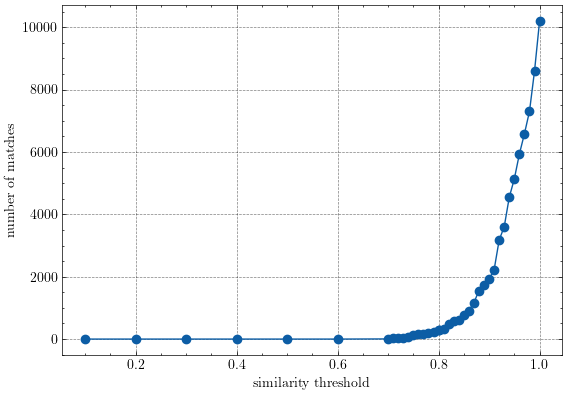
\includegraphics[width=\textwidth]{countries_20-most-popul_thresholds.png}
%         \caption{Similarity threshold variation for all \textsf{semsim} patterns}
%         \label{fig:countries_20-most-popul_thresholds}
%     \end{subfigure}
%     \begin{subfigure}[t]{0.9\textwidth}
%         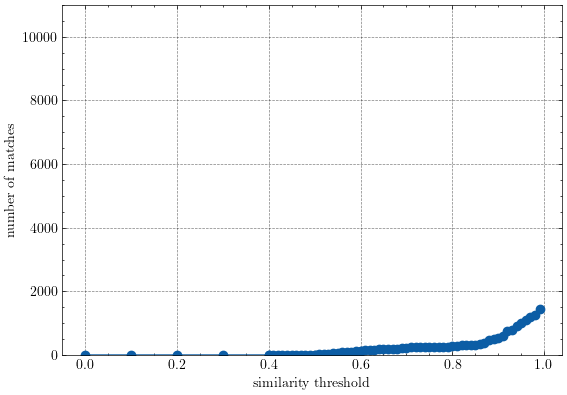
\includegraphics[width=\textwidth]{countries_20-most-popul_thresholds-countries.png}
%         \caption{Similarity threshold variation only for \textsf{SOURCE} and \textsf{TARGET} (country) \texttt{semsim} patterns}
%         \label{fig:countries_20-most-popul_thresholds-countries}
%     \end{subfigure}
%\caption{Number of matches for conflict pattern in relation to similarity threshold}
%\label{fig:case-study-conflict-countries-1}   
%\end{figure}
%
%\begin{figure}
%     \centering
%     \begin{subfigure}[t]{0.9\textwidth}
%         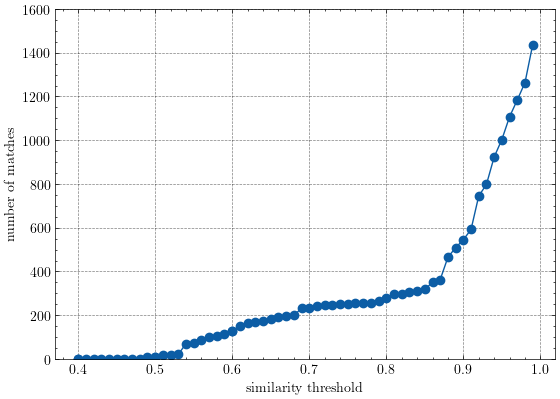
\includegraphics[width=\textwidth]{countries_20-most-popul_thresholds-countries_greater-0.4.png}
%     \end{subfigure}
%\caption{Number of matches for conflict pattern in relation to similarity threshold with threshold variation for \textsf{SOURCE} and \textsf{TARGET} (i.e. COUNTRIES) \texttt{semsim} patterns in the range \(0.4 >=\) threshold \(< 1.0\) (and y-axis limited to 2000 results)}
%\label{fig:case-study-conflict-countries-2}   
%\end{figure}

%\subsection{Qualitative Results}
%
%
%\begin{sidewaystable}
%%    \centering
%    \caption{hyper dyper table}
%
%\begin{tabular}{L{4cm}L{2cm}L{5cm}L{3cm}L{5cm}L{3cm}}
%\toprule
%Scenario Name & Pattern & Samples & Variable Threshold & Reference Edges & Ref. Edges Source \\
%\midrule
%1\_original-pattern & Pattern X & Erdogan slams ridicule of 'Muslims discovered Americas' claim\newline Iran forces 'kill Kurdish rebels on Iraq border\newline Ukraine Accuses Russia of Invasion & -/- & -/- & -/- \\
%2-1\_semsim-fix\_preds & Pattern X & Pakistani police kill feared militant leader in mysterious pre-dawn shootout\newline Al-Shabaab militants claim responsibility for deadly attack on Garissa University College in Kenya\newline Casualties as Congo troops, UN forces fight rebels & 'preds': 0.19\newline Percentile: 50 & -/- & -/- \\
%2-2\_semsim-fix\_preps & Pattern X & Iranian police have arrested merchants for selling clothing that featured the flags of the United States and Britain, two longtime foes of the Islamic republic\newline Syrian Air Force Strikes kill 38 ISIS fighters\newline Seven Libyan soldiers killed fighting off Islamists near Benghazi: source & 'preps': 0.54\newline Percentile: 50 & -/- & -/- \\
%\bottomrule
%\end{tabular}
%
%\end{sidewaystable}

%\begin{table*}
%\
%\end{table*}

% ========== 
\chapter{Conclusion}

\chapter{Future Work}
\section{Implementation Improvements}
implemnt multiprocessing, i.e. server process for both hypergraph and semsim matchers. other option would be to leverage python shared memory capabilities but is likely to be less stable and has less scaling potential

\section{Further Evaluations}



\printbibliography


\end{document}
